\documentclass[12pt]{article}

\usepackage[french]{babel}
\usepackage[utf8x]{inputenc}
\usepackage[OT1]{fontenc}

\usepackage{graphicx}
\usepackage{verbatim}
\usepackage{amsfonts}
\usepackage{comment}


\title{Aperçu d'une architecture de Reservoir Computing\\Les Echo State Networks}
\author{Théo \bsc{Biasutto--Lervat}}
\date{}

\begin{document}
\maketitle


\section{Introduction}
Le \textit{Reservoir computing} (RC) est une alternative à la méthode de descente du gradient pour entraîner les \textit{recurrent neural network} (RNN), une architecture de réseau de neurones artificielles où les connections synaptiques peuvent former des cycles. Cela entraîne l'apparition d'états internes au sein du réseau, lui permettant d'adopter un comportement temporel dynamique.\newline
Un \textit{Echo state network} est un RNN possèdant une couche cachée, le réservoir, avec un faible nombre de synapse dont les poids sont générés aléatoirement. Le poid des neurones de sortie est l'unique sous-ensemble du réseau qui sera entraîné, bien souvent à l'aide d'une régression linéaire.\newline
Pour que l'approche ESN fonctionne, le réservoir doit satisfaire \textit{l'echo state property}: l'état d'un réservoir ne doit dépendre que des données entrées au court du temps. Pour un réservoir assimilant une grande quantitée de donnée, son état interne ne doit donc plus dépendre de l'initialisation.


\section{Formalisation}
Considérons un réseaux de neurones en temps discret, avec K neurones d'entrée, N neurones internes, et L neurones de sortie.\newline
\begin{center}
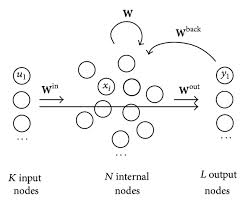
\includegraphics[scale=0.5]{esn.jpeg}
\end{center}
\begin{description}
\item[$u(n)$ :] vecteur $\in \mathbb{R}^{K}$, activations des neurones d'entrée à l'instant n
\item[$x(n)$ :] vecteur $\in \mathbb{R}^{N}$, activations des neurones internes à l'instant n
\item[$y(n)$ :] vecteur $\in \mathbb{R}^{L}$, activations des neurones de sortie à l'instant n
\item[$W^{in}$ :] $N \times K$ matrice $\in \mathbb{R}$, poids des synapses d'entrée
\item[$W$ :] $N \times N$ matrice $\in \mathbb{R}$, poids des synapses internes
\item[$W^{out}$ :] $L \times (K + N + L)$ matrice $\in \mathbb{R}$, poids des synapses de sortie
\item[$W^{back}$ :] $N \times L$ matrice $\in \mathbb{R}$, poids des synapses de \textit{feedback}
\item[$\alpha$ :] le taux de fuite
\end{description} 

\section{Fonctionnement}
\subsection{Généralité}
Dans le cas d'un apprentissage supervisé, c'est à dire dont les résultats sont connu à l'avance, voici les différentes équations décrivant le fonctionnement de l'ESN.\newline
\paragraph{L'état interne}
\begin{center}
$x(n) = f(W^{in}u(n) + Wx(n-1) + W^{back}y(n-1) )$
\end{center}
où $f=(f_{1},...,f_{N})$ sont les fonctions d'activations des neurones du réservoir.\newline
Dans le cas d'un ESN sans synapse de \textit{feedback}, avec biais et avec pour fonctions d'activation $\tanh$, nous obtenons
\begin{center}
$x(n) = (1-\alpha)x(n-1) + \alpha\tanh(W^{in}[1;u(n)] + Wx(n-1))$
\end{center}
\paragraph{La sortie}
\begin{center}
$y(n)= W^{out}[1;u(n);x(n)]$
\end{center}
\paragraph{Apprentissage de $W^{out}$}
\begin{center}
$W^{out} = Y^{target} X^\top (XX^\top + \beta I)^{-1}$
\end{center}
où $\beta$ est le coefficient de régularisation (A COMPLETER).

\subsection{Mise en oeuvre}
\begin{enumerate}
\item Générer le réservoir ($W^{in}$, $W$, $\alpha$);
\item Utiliser le corpus d'apprentissage $u(n)$ et collecter $x(n)$;
\item Calculer $W^{out}$ en minimisant la différence entre  $y(n)$ et $y^{target}(n)$;
\item Utiliser les nouvelles données $u(n)$, obtenir  $y(n)$ avec $W^{out}$.
\end{enumerate}

\section{Astuces}
\subsection{Generation du réservoir}
\paragraph{Taille du réservoir}
L'entrainement et l'utilisation d'un ESN est peu couteux à côté des autres approches de RNN, ce qui nous permets de créer de grand réservoir, avec un ordre de grandeur de $10^{4}$ neurones. Le réservoir peut cependant être trop gros si la tâche est triviale et qu'il n'y a pas assez de donnée disponible dans le corpus d'apprentissage.\newline
Dans \textit{A Pratical Guide to Applying Echo State Network}, il est dit :
\begin{itemize}
\item Pour des tâches complexes, utiliser un réservoir aussi gros que vous le pouvez.
\item Choisir les paramètres pour de petit réservoir, puis les mettres à l'échelle pour de plus gros.
\item N doit être au moins égal à l'estimation de valeur indépendante que le réservoir doit mémoriser depuis les entrées pour résoudre la tâche.
\end{itemize}

\paragraph{Parcimonie du réservoir}
Une grande partie des éléments de $W^{in}$ doivent être nul. En général, la parcimonie du réservoir affecte peu les performances du réseau de neurone.\newline
Dans \textit{A Pratical Guide to Applying Echo State Network}, il est dit :
\begin{itemize}
\item Connecter chaque neurone à un petit nombres de neurones, indépendament de la taille du réservoir. Profiter de cette parcimonie pour accélerer les calculs.
\end{itemize}

\paragraph{Distribution des éléments non-nuls}
Une grande partie des éléments de $W$ sont nuls, et la distribution des éléments non-nuls peut s'effectuer de différente façon : \textit{symmetrical uniform}, \textit{discrete bi-valued}, \textit{normal distribution centered around zero}, \textit{Gaussian distribution}.\newline
La distribution Gaussienne et normal donne virtuellement les mêmes résultats, la distribution \textit{discrete bi-valued} semble moins efficace, mais peut faciliter l'analyse du réservoir lors de son exécution.

\paragraph{Rayon spectral}
Un des paramètres majeurs d'un ESN est le rayon spectral de la matrice $W$. Généralement, une fois la génération de $W$ effectuée, la matrice est divisée par $\rho(W)$ pour assurer un rayon spectral unitaire. Le rayon spectral détermine à quelle vitesse l'influence d'une entrée disparait du réservoir, et à quel point l'état interne du réservoir est stable.\newline
Dans \textit{A Pratical Guide to Applying Echo State Network}, il est dit :
\begin{itemize}
\item $\rho(W) < 1$ assure dans la propriété \textit(echo state) dans la plupart des situations.
\item Le rayon spectral optimale est souvent plus grand lors de tâche nécessitant une grande mémoire des entrées.
\end{itemize}

\paragraph{Redimensionnement des entrées}
Autre paramètre essentiel d'un ESN, la matrice $W^{in}$ détermine la linéarité de la réponse du réservoir. Pour des tâches très linéaire, $W^{in}$ devrait être peuplé de faible valeur. Lorsque $W^{in}$ possède de forte valeur, les neurones ont tendances à agir comme des commutateurs binaires. De plus, l'échelle de $W^{in}$ et celle de $W$ détermine respectivement comment l'état interne $x(n)$ dépent de l'entrée $u(n)$ et de $x(n-1)$.\newline
Dans \textit{A Pratical Guide to Applying Echo State Network}, il est dit :
\begin{itemize}
\item Mettre à l'échelle $W^{in}$ uniformément, pour limiter le nombre de paramètre de l'ESN. Cependant, par souçi de performance, il est possible de redimmensionner la première colonne de $W^{in}$ (le biais) séparement, et de redimmensionner les autres colonnes séparement si les éléments de $u(n)$ contribue différement à la tâche.
\item Il est conseillé de normaliser les données, ce qui peut aider à borner $u(n)$ et ainsi éviter des aberrations. Par exemple, appliquer $tanh(.)$ à $u(n)$ si celui ci n'est pas borné.
\item Le redimensionnement des entrées régule la quantitée de non-linéarité de $x(n)$ (augmente aussi avec $\rho(W)$), et l'effet de l'entrée courante sur $x(n)$ par rapport aux entrées précédantes (proportionnellement à $\rho(W)$).
\end{itemize}

\paragraph{Taux de fuite}
Le troisième paramètre primordial des ESN, le taux de fuite peut être compris comme la vitesse de la dynamique de mise à jour du réservoir, mais aussi comme l'interval de temps entre deux consecutives \textit{timestep} de la réalisation discrète.\newline
Dans \textit{A Pratical Guide to Applying Echo State Network}, il est dit :
\begin{itemize}
\item Le taux de fuite $\alpha$ doit correspondre à la vitesse de la dynamique de $u(n)$ et/ou $y^{target}(n)$.
\end{itemize}

\subsection{Apprentissage}
Bientôt...

\begin{comment}
\paragraph{Script}
\begin{verbatim}
network = ESN()

network.setGenerationStrategy(genStrat)
network.generateReservoir(K, N, L, a)

for i=0; i<initTransient; i++ :
 network.feed(u[i])

X = zeros( (1+K+N, len(data)-initTransient ) )
for i=0; i<len(data); i++ :
 network.feed(data[i+initTransient])
 X[:, i] = vstack( (1, data[i+initTransient], network.x) )[:, 0] 

network.setLearningStrategy(learnStrat)
network.learn(ytarget, X)
\end{verbatim}

\paragraph{Classes utilitaires}
\begin{verbatim}
def class ESN :
 def setGenerationStrategy(self, genStrat):
  self.genStrat = genStrat

 def setLearningStrategy(self, learnStrat):
  self.learnStrat = learnStrat

 def generateReservoir(self, K, N, L, a):
  self.Win = genStrat.generateWin(K, N)
  self.W = genStrat.generateW(N)
  self.a = a
  self.x = zeros((N, 1))

 def learn(self, ytarget, x):
  self.Wout = learnStrat.learnWout(ytarget, x)
  
 def feed(data):
  self.x = (1-a)*x + a*tanh( dot(Win, vstack((1, u))) + dot(W, x) )
\end{verbatim}

\end{comment}

\end{document}